\section{Theory}
A device that translates a continuous physical quantity (typically voltage) to a digital number that indicates
the quantity’s amplitude is known as an analog-to-digital
converter (ADC). A DAC, on the other hand, accepts a
binary number and generates an analog voltage or current
signal. They are frequently employed in digital systems in
conjunction to offer a comprehensive interface with analog devices and output devices for control systems.

\subsection{Digital to Analog Converter}
A Digital to Analog Converter (DAC) has several binary inputs and one output. In general, a DAC’s number
of binary inputs will be a power of two. DACs are classified into two types: weighted resistor DACs and $R/2R$
ladder DACs. The addition of digital inputs (0 or 1,
where 1 equates to 5 volts) in a weighted resistor produces analogue output, which can be added with varied
weights depending on their position in the binary number. However, because of the large number of bits, this
form of circuit needs a large number of precise resistors.
Using an $R-2R$ ladder network in the inverting adder circuit, the $R-2R$ Ladder DAC overcomes this disadvantage
and delivers an analogue output that is almost identical
to the digital (binary) input. 

The performance of DAC is
characterized by the following:\\

\begin{itemize}
    \item \textbf{Resolution:} The resolution of a DAC is determined by the number of bits (N). The resolution is the lowest output increment that the DAC can produce. The resolution of an 8-bit DAC is 8 bits, or one part in $2^8$. This yields a percentage of $0.39\%$.\\
    \item \textbf{Linearity/ Linear Errors:} The maximum permitted variation from an ideal straight line drawn between the zero-scale and full-scale outputs is defined as linearity. It is frequently expressed as a percentage or as a fraction of an LSB. For an 8-bit DAC, ($\frac{1}{2}$) LSB linearity equates to $0.195\%$.\\
    \item \textbf{Monotonicity:} If each digital code increase generates an output equal to or greater than the preceding code, the DAC is monotonic. A DAC is often anticipated to be monotonic to increments as tiny as an LSB, but its monotonicity is determined by the smallest increment for which the DAC stays monotonic.\\
    \item \textbf{Settling time:} The settling time is calculated as the time it takes from the instant a digital input code changes to the time the analogue output achieves its matching new value within a given error band. Typically, the output is anticipated to settle within a $\frac{1}{2}$ LSB error range. Typically, the worst-case settling time is evaluated between the zero-scale and full-scale codes.\\
    \item \textbf{Accuracy:} The maximum divergence between the actual converter output and the ideal converter output is defined as absolute accuracy. The greatest variation after removing gain and offset errors is referred to as relative accuracy.
\end{itemize}
% \vspace{-1em}
\subsection{Analog to Digital Converter}

% \begin{figure}[H]
%     \centering
%     \label{theory:1}
%     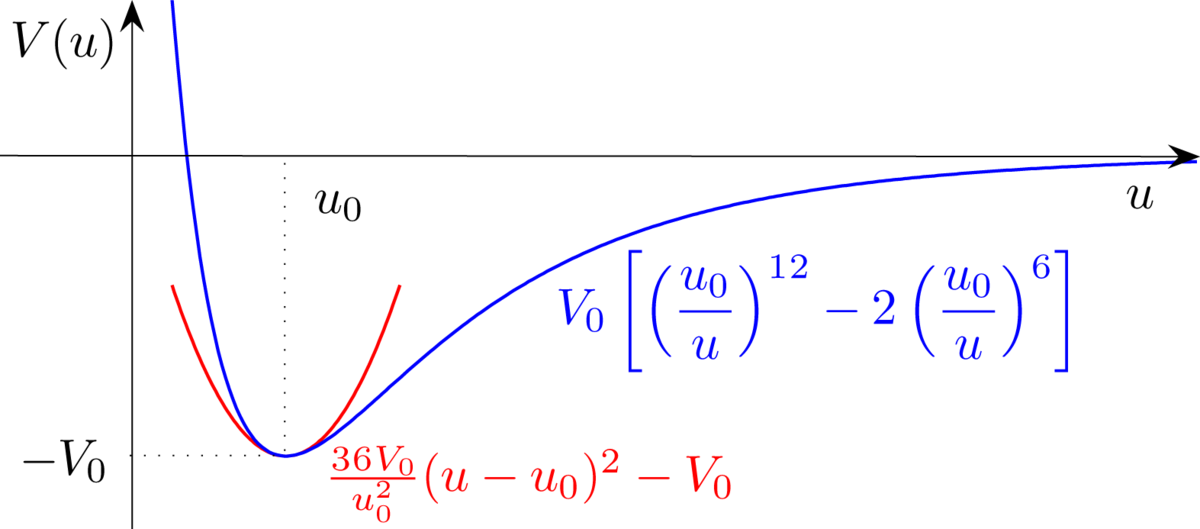
\includegraphics[width=0.6\columnwidth]{images/theory1.png}
%     \caption{Analog to Digital Converter}
% \end{figure}

There are many different ways to take an analog voltage signal and convert it into an equivalent digital signal. While many analog-to-digital converter chips are available, it is possible to build a simple ADC using discrete components.

One simple and easy way is by using parallel encoding, also known as flash, simultaneous, or multiple comparator converters, in which comparators are used to detect different voltage levels and output their switching state to an encoder.


% ======================================================
\section{Experimental Setup}

\subsection*{Apparatus}

\begin{enumerate}
    \item Resistors: 330 $\Omega$, 1 k$\Omega$, 2 k$\Omega$, R, and 2R (as per the $R/2R$ ladder requirements)
    \item 74147 priority encoder IC
    \item \verb|7447| binary-to-BCD decoder IC
    \item LM339 comparator IC
    \item Digital multimeter
    \item DC power supply
    \item Breadboard and connecting wires
    \item LEDs
    \item Common anode BCD display
\end{enumerate}

\subsection{4 bit R/2R ladder DAC using 741 op-amp}
\begin{figure}[H]
    \centering
    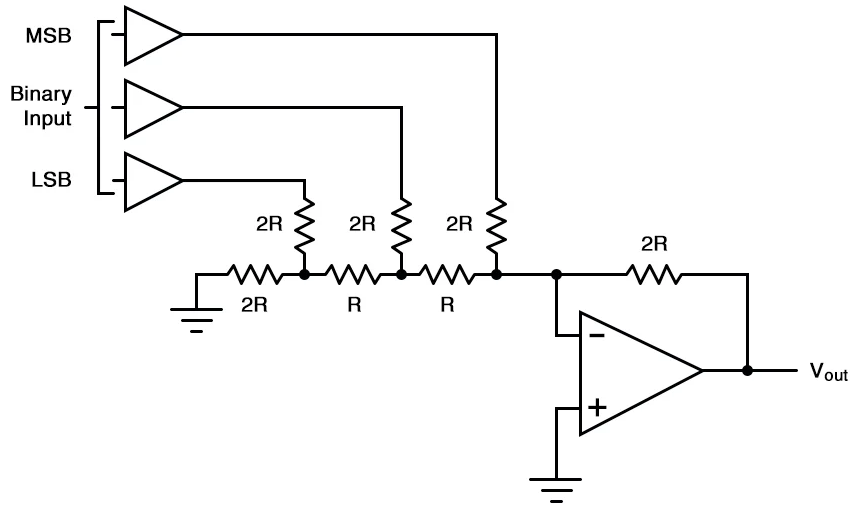
\includegraphics[width=1\columnwidth]{images/th1.png}
    \caption{ Circuit diagram for 3-bit digital to analog conversion }
    \label{obj:1}
\end{figure}
The DAC circuit consists of a 3-bit R/2R ladder DAC using 741 op amp by choosing components appropriately and testing the circuit. The figure is depicted above. The output voltage of the DAC circuit is given by:
		
\begin{align}\label{eq1} V_{out} = \frac{-R_F}{R}\left( \frac{d_1}{2^1} + \frac{d_2}{2^2} + \frac{d_3}{2^3} \right)\end{align}

where $d_1$ is M.S.B and $d_3$ is L.S.B. In the above circuit, feedback resistance $R_f=2R$. The output impedance of the $R-2R$ network is always R for any number of bits in the network. This Another advantage of the circuit is that it simplifies the design of circuits that use DAC, such as filtering, amplification, etc. For a 4-bit DAC, the equation becomes
\begin{align}\label{eq2} V_{out} = \frac{-R_F}{R}\left( \frac{d_1}{2^1} + \frac{d_2}{2^2} + \frac{d_3}{2^3} \frac{d_4}{2^4} \right)\end{align}

\subsection{ADC circuit to convert a 2-bit digital input to analog output}
\hyperref[obj:2]{Figure 3} depicts the conversion's circuit diagram. This circuit employs an \verb|LM339| comparator and \verb|74147| priority encoders. The \verb|LM339| comparator chip compares the analogue input from the DC power source with a reference voltage before passing it to the \verb|74147| priority encoder circuit. The binary output from the \verb|74147| chip may then be translated to BCD (Binary coded decimal) format and shown as a decimal digit on a common cathode 7-segment BCD display using the \verb|7447| device. Use three of the four available comparators in \verb|LM339|.

Digital binary output can be produced through $D_0$, $D_1$, $D_2$ and $D_3$. It should be noted that the \verb|LM339| is a quad comparator integrated circuit. Because it has an open collector, it requires pull-up resistors at the comparator's output, as illustrated in \hyperref[obj:2]{Figure 3}. Pull-up resistors of $3k\ohm$ are recommended. When utilising the \verb|LM339| chip, always connect a $1k\ohm$ resistor in series with the LEDs. The supply voltage to the \verb|LM339| can be as high as $15V$. Adjust the reference voltage as needed. Before connecting the ADC circuit, learn how the \verb|LM339| works by connecting one of the comparators and testing the output. \verb|74147| is a priority encoder with a range of 10 to 4. This IC's input and output are both low. The unused pins should be pulled up to $5V$.
\begin{figure}[H]
    \centering
    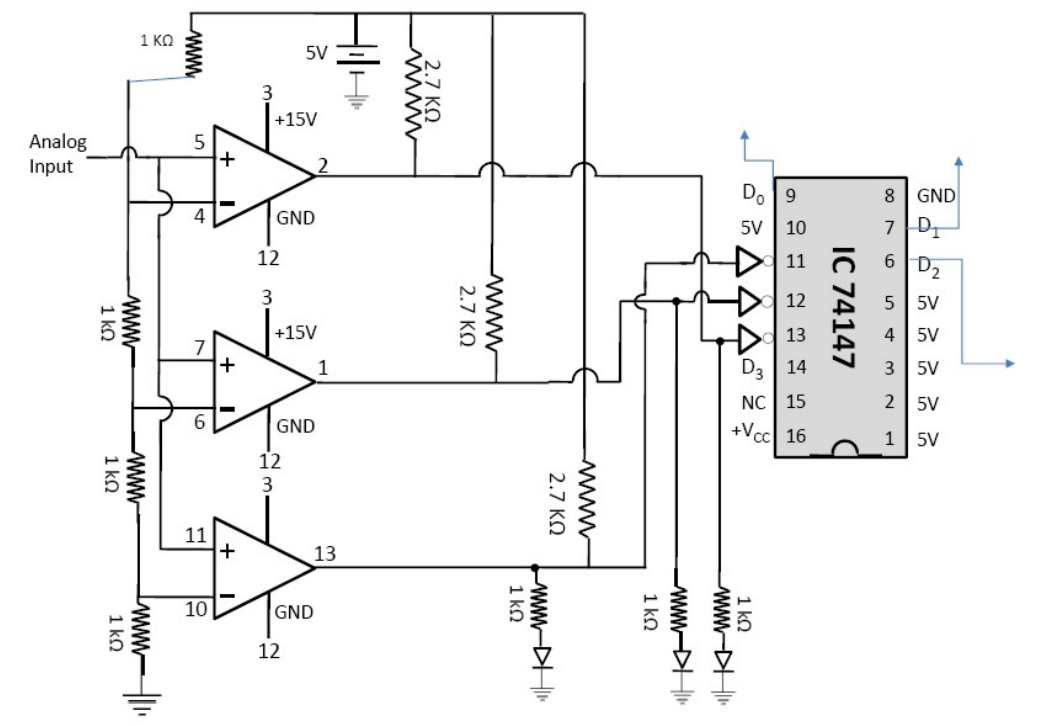
\includegraphics[width=1\columnwidth]{images/th2.png}
    \caption{ Circuit diagram for 2-bit binary Analog to Digital conversion }
    \label{obj:2}
\end{figure}

\subsubsection*{Conversion of the binary display to decimal display}
After converting analog voltage to binary number, it can be converted to binary coded decimal and displayed on a BCD display. $\verb|7447|$ is an input active high IC and output active low IC. The output of the $\verb|7447|$ must be connected to BCD display via a $330\ohm$ resistor.